\subsection{Setting Up}


\begin{frame}[fragile]
  \frametitle{Who Are You?}

  Your name and email address become part of the commit message 
  \begin{itemize}
  \item Global configuration stored in $\sim$\verb#/.gitconfig#. Either
    open in your favorite editor to add
    \begin{shell}
    [user]
        name = Your Name
        email = you@host.com
    \end{shell}
  \item or via the command line:
    \begin{shell}
git config --global user.name "Your Name"
git config --global user.email you@host.com
    \end{shell}    
  \end{itemize}

\end{frame}


\begin{frame}[fragile]
  \frametitle{Trac Account}
  
  To contribute to Sage, you need 
  \begin{itemize}
  \item a trac account, see instructions at \url{http://trac.sagemath.org}
  \item upload your ssh \emph{public} key to the trac server
  \item This is described in detail in
    \url{http://sagemath.github.io/git-developer-guide/trac.html#authentication},
    a temporary copy of the new developer guide.
  \end{itemize}
  
\end{frame}



\subsection{Using Git for Sage}


\begin{frame}
  \frametitle{Obtaining the Sage Sources}
  
  \begin{itemize}
  \item 
    Download the Sage git repository from github:\\
    \cmd{git clone git://github.com/sagemath/sage.git}
  \item 
    Setup the ``trac'' remote:\\
    {
      \cmd{cd sage}
      \cmd{git remote add trac}\\
      \hfill
      \cmd{ssh://git@trac.sagemath.org:2222/sage.git -t master}
    }
  \item Note: the \cmd{-t master} means to only fetch the master
    branch by default 
    \begin{itemize}
    \item Pro: Avoids downloading all branches on trac; Faster and
      less clutter
    \item Con: You have to tell git which branches to download
    \end{itemize}
  \end{itemize}
\end{frame}




\begin{frame}
  \frametitle{Downloading a Branch from Trac}

   \begin{alertblock}{Temporary change}
     You should use the \cmd{public/sage-git/master} branch for
     now. When the git transition is finished, it well be just
     \cmd{master}.
   \end{alertblock}
   
   So, first get this branch:
   \begin{itemize}
   \item 
     Tell git which branch to download:\\
     \cmd{git fetch trac public/sage-git/master}
   \item 
     Create a new local branch from what you just downloaded:\\
     \cmd{git checkout -b trac\_master FETCH\_HEAD}
   \end{itemize}

   Then build Sage as usual (run \cmd{make})
\end{frame}


\subsection{Integration with Sage Trac}

\begin{frame}
  \frametitle{Uploading Changes}

  \begin{itemize}
  \item Now edit files and commit changes. Just like with any other git
    repository.
  \item If you have a (new or existing) ticket, fill in the
    ``Branch:'' field with the name that you will be using to upload.
  \item The remote branch name must be \cmd{u/user/description}, where
    \begin{itemize}
    \item \cmd{user} is your trac username
    \item \cmd{description} is a free-form short description (and can
      include further slashes)
    \end{itemize}
  \item 
    When you are ready to share, upload to trac:\\
    \cmd{git push --set-upstream trac}\\
    \hspace{2cm}\cmd{my\_branch:u/user/description}
  \item 
    Slightly different push command for subsequent uploads:\\
    \cmd{git push trac HEAD:u/user/description}
  \end{itemize}
\end{frame}



\begin{frame}
  \frametitle{Using Trac}

  \begin{itemize}
  \item When you push to a trac ticket, the ``Commit:'' field on the
    trac ticket is automatically filled out.
  \item The ``Branch:'' field is color coded:
    \begin{itemize}
    \item \textcolor{green}{Green} means that it applied cleanly to the current master.
    \item \textcolor{red}{Red} means that there is a conflict.
    \end{itemize}
  \item If you click on the ``(Commits)'' link under/next to the
    branch, you can see the list of commits.
  \item Download any branch for the first time as on the ``Downloading
    a Branch from Trac'' slide.
  \item To get changes, use \cmd{git pull trac u/user/description}
  \end{itemize}
\end{frame}


{
  \usebackgroundtemplate{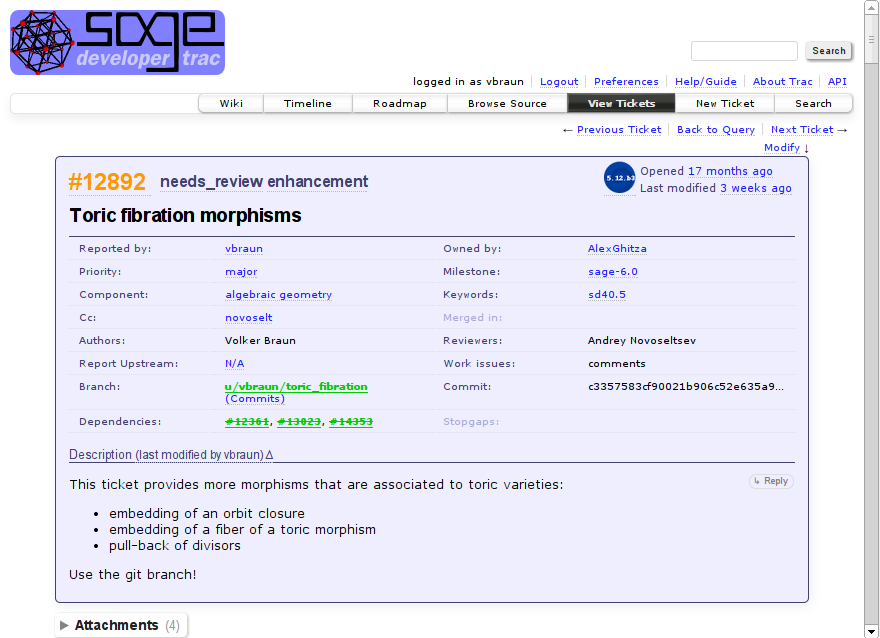
\includegraphics[width=\paperwidth]{images/trac_screenshot}}
  \begin{frame}[plain]
  \end{frame}
}




\begin{frame}[fragile]
  \frametitle{Merging vs.\ Rebasing}

  While you are working on \cmd{my\_branch}, Sage development
  continues.
\begin{verbatim}
             X---Y---Z my_branch
            /
       A---B---C---D master
\end{verbatim}
  Two ways to update:
  \begin{itemize}
  \item Merge: \cmd{git merge master}
\begin{verbatim}
             X---Y---Z---W my_branch
            /           /
       A---B---C-------D master
\end{verbatim}
  \item Rebase: \cmd{git rebase master}
\begin{verbatim}
                     X'--Y'--Z' my_branch
                    /
       A---B---C---D master
\end{verbatim}
  \end{itemize}
  
\end{frame}





\begin{frame}[fragile]
  \frametitle{Rebasing}
  
    \begin{itemize}
    \item Rebase: \cmd{git rebase master}
\begin{verbatim}
                     X'--Y'--Z' my_branch
                    /
       A---B---C---D master
\end{verbatim}
    \item Pro: Clean history.
    \item Con: Since the SHA1 hash includes the hash of the parent,
      all commits change.
    \item Only ever use rebase if nobody else has used one of your
      \texttt{X}, \texttt{Y}, \texttt{Z} commits to base their
      development on.
    \item Only rebase commits that you have not yet pushed to trac.
  \end{itemize}
  
\end{frame}





\begin{frame}[fragile]
  \frametitle{Merging}
  
    \begin{itemize}
  \item Merge: \cmd{git merge master}
\begin{verbatim}
             X---Y---Z---W my_branch
            /           /
       A---B---C-------D master
\end{verbatim}
      \item Pro: None of the existing commits changes
      \item Con: Introduces a new commit \texttt{W} that will be in the
        \cmd{git log} history forever.
      \item When you push to trac, the extra commit propagates to your
        collaborators. 
      \item When in doubt, use merge instead of rebase.
  \end{itemize}
  
\end{frame}







%%% Local Variables:
%%% TeX-master: "talk.tex"
%%% eval: (TeX-PDF-mode 1)
%%% End:

